% !TEX encoding = UTF-8
\documentclass[fontsize=12pt,paper=letter,twoside]{scrartcl}
% Various imports and themes
\usepackage[top=4cm,bottom=4cm,left=3cm,right=3cm,asymmetric]{geometry}
%\geometry{landscape}
  % Activate for for rotated page geometry
%\usepackage[parfill]{parskip}    
  % Begin paragraphs with an empty line rather than an indent
\usepackage[table,xcdraw]{xcolor}
\usepackage{graphicx}

\usepackage{amsmath}
\usepackage{amssymb}
\usepackage{epstopdf}
\DeclareGraphicsRule{.tif}{png}{.png}{`convert #1 `dirname #1`/`basename #1 .tif`.png}
% Listings needs package courier
\usepackage{listings} % Needs 
\usepackage{courier}

\usepackage[framemethod=TikZ]{mdframed}
\usepackage{url}

\usepackage{sty/bsymb} %% Event-B symbols
\usepackage{sty/eventB} %% REQ and ENV
\usepackage{sty/calculation}
\usepackage{sty/mathpartir}

% \usepackage{sty/tikz-uml}


%Maths
\usepackage{amssymb,amsmath}
\def\Fl{\mathbb{F}}
\def\Rl{\mathbb{R}}
\def\Nl{\mathbb{N}}
\def\Bl{\mathbb{B}}
\def\St{\mathbb{S}}
\newcommand{\ovr}{\upharpoonright}
\newcommand{\var}[1]{\textit{#1}}
%Useful definitions
\newcommand{\mv}[1]{\textit{m\_#1}}
\newcommand{\cv}[1]{\textit{c\_#1}}
\newcommand{\degree}[1]{^{\circ}\mathrm{#1}}
%\newcommand{\comment}[1]{{\footnotesize \quad\texttt{--}\textrm{#1}}}
\newcommand{\im}[1]{i\texttt{-\!#1}}

\usepackage[headsepline]{scrpage2}
\pagestyle{scrheadings}
\ihead[]{\small EECS4312 Report1}
\ohead[]{\small \thepage}
\cfoot[]{}
\ofoot[]{}


%%%%PVS environment%%%%%%%%%%%%%%%%%%%
\lstnewenvironment{pvs}[1][]
    {\lstset{#1,captionpos=b,language=pvs,
    mathescape=true,
    basicstyle=\small\ttfamily,
    numbers=none,
    frame=single,
    % numberstyle=\tiny\color{gray},
    % backgroundcolor=\color{lightgray},
    firstnumber=auto
    }}
    {}
 %%%%%%%%%%%%%%%%%%%%%%%%%%%%%%%%
 
%%%%PVS environment%%%%%%%%%%%%%%%%%%%
\lstnewenvironment{events}[1][]
    {\lstset{#1,captionpos=b,language=events,
    mathescape=true,
    basicstyle=\small\ttfamily,
    numbers=none,
    frame=single,
    % numberstyle=\tiny\color{gray},
    % backgroundcolor=\color{lightgray},
    firstnumber=auto
    }}
    {}
 %%%%%%%%%%%%%%%%%%%%%%%%%%%%%%%%
 
%%%%Verbatim environment%%%%%%%%%%%%%%%%%%%
\lstnewenvironment{code}[1][]
    {\lstset{#1,captionpos=b,
    mathescape=true,
    basicstyle=\scriptsize\ttfamily,
    numbers=none,
    frame=single,
    comment=[l][\color{red}]{--},
    % keywords = [1]{"->"},
    % numberstyle=\tiny\color{gray},
    % backgroundcolor=\color{lightgray},
    firstnumber=auto
    }}
    {}

% \newenvironment{boxed}[1]
%    {\begin{center}
%    #1\\[1ex]
%    \begin{tabular}{|p{0.9\textwidth}|}
%    \hline\\
%    }
%    { 
%    \\\\\hline
%    \end{tabular} 
%    \end{center}
%    }
 %%%%%%%%%%%%%%%%%%%%%%%%%%%%%%%%
 
 %Text in a box
\newenvironment{textbox}
    {\begin{center}
    \begin{tabular}{|p{0.9\textwidth}|}
    \hline\\
    }
    { 
    \\\\\hline
    \end{tabular} 
    \end{center}
    }

\usepackage{hyperref}

%Highlight \hl{}
\usepackage{soul}

\usepackage{enumitem}
\newlist{mylist}{itemize}{1}
\setlist[mylist]{label=\textbullet,leftmargin=1cm,nosep}

\usepackage{multirow}

% Reduce space between figure and caption
%\usepackage{caption}
%\captionsetup[table]{font=small,skip=0pt}     %% Adjust here
%or equivalently 
\usepackage[font=small,skip=4pt]{caption}

% Indent equations
%\setlength{\mathindent}{1cm}

% Set the header

%\afterpage{\clearpage}
\usepackage{afterpage}
\usepackage{fancyvrb}

% Allow better table placement?
\renewcommand\floatpagefraction{.9}
\renewcommand\topfraction{.9}
\renewcommand\bottomfraction{.9}
\renewcommand\textfraction{.1}   
\setcounter{totalnumber}{50}
\setcounter{topnumber}{50}
\setcounter{bottomnumber}{50}
\usepackage{morefloats}
\usepackage[section]{placeins}

\newcommand{\pre}[1]{{#1}_{-1}}
\newtheorem{defn}{Definition}%[section]
\newtheorem{lemma}{Lemma}%[section]
\newtheorem{theorem}{Theorem}%[section]

%Sequents
\usepackage{bussproofs}

% Hide sections
\newif\ifhideproofs
%\hideproofstrue %uncomment to hide proofs

% Needed for TLA
% \input{tla/tla-style.tex} % style file for TLA
% Reduce space around equations
\setlength{\abovedisplayskip}{3pt}
\setlength{\belowdisplayskip}{3pt}


 
\usepackage{pdfpages}
%%%%%%%%%%%%%%%%%%%%%%%%%%%%%%%%%%%%%%%%%%%%%%%%%%%%%%%%%%%%%%%%%%%%%%%%%
\begin{document}
%%%%%%%%%%%%%%%%%%%%%%%%%%%%%%%%%%%%%%%%%%%%%%%%%%%%%%%%%%%%%%%%%%%%%%%%%
% Title and Authors
\newcommand{\mytitle}{
	EECS2311-W20 Project: Venn Create\\ Requirements Document
}
\ihead[]{\small \mytitle}
\title{\mytitle}
\subtitle{Group 18}
\author{
	Chidalu Agbakwa (216337784) \and
	Jihal Patel (216376436) 	\and
	Shangru Li (214488993) 		\and
	Robert Suwary (215446016)
}
% Display a given date or no date
\date{\today}
\maketitle
%%%%%%%%%%%%%%%%%%%%%%%%%%%%%%%%%%%%%%%%%%%%%%%%%%%%%%%%%%%%%%%%%%%%%%%%%
\newpage
\vspace*{2in}
\begin{center}
	\huge{\textbf{Requirements Document}:\\ Venn Create}
\end{center}
\newpage
%%%%%%%%%%%%%%%%%%%%%%%%%%%%%%%%%%%%%%%%%%%%%%%%%%%%%%%%%%%%%%%%%%%%%%%%%
\newpage
\tableofcontents
\newpage
\listoffigures
\listoftables
%%%%%%%%%%%%%%%%%%%%%%%%%%%%%%%%%%%%%%%%%%%%%%%%%%%%%%%%%%%%%%%%%%%%%%%%%
\newpage
\section{Purpose of Venn Create}
The system under development is a desktop software that can draw customizable
Venn diagrams.

\begin{figure}[hbt]
	\begin{center}
		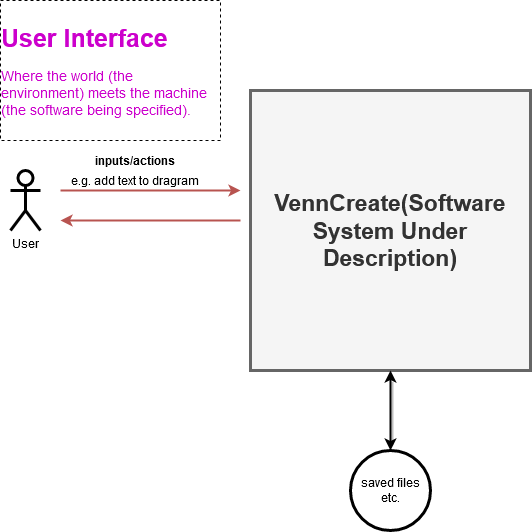
\includegraphics[width=\textwidth]{images/context-diagram.png}
	\end{center}
	\caption{Context Diagram of Venn Create}
\end{figure}

A Venn diagram (also called primary diagram, set diagram or logic diagram) is a diagram that shows all possible logical relations between a finite
collection of different sets. It is a great way to present relationships
between sets of objects, such as set intersection or set difference.

By using Venn Create, user can easily create Venn diagrams with customized
labels, in different size and shape. Which can be used to compare and
contrast two or more objects, events, people, or concepts. Clearly
illustrating the differences and similarities between different entities.

Venn Create provides a user-friendly interface, so that new users will
be able to use the application with minimum efforts. In addition,
the application provides essential functionalities, such as export current Venn diagram to a local file or import an existing Venn diagram from a saved file.
 

%%%%%%%%%%%%%%%%%%%%%%%%%%%%%%%%%%%%%%%%%%%%%%%%%%%%%%%%%%%%%%%%%%%%%%%%%
\newpage
\section{Document Conventions and Dictionary}

\begin{itemize}
	\item \textbf{Venn diagram}: a diagram that shows all possible logical relations between a finite collection of different sets.
	\item \textbf{Test Mode}: a testing mode for the software Venn Create, where the users can import a .txt file with information that they would like to be “tested” on and VennCreate will give them a test.
	\item \textbf{Shape Scene}: The main scene that Venn Create will be operated in. Displays the Venn Circles, text labels and receives user command through inputs.  
	\item \textbf{Word Bank}: a place that stores all the contents of the text label added to the current Venn diagram. Which is shown on the Navigation Bar on the left side of the main scene. Users will be able to remove a specific item from the Word Bank of their choice, or empty the Word Bank.
	\item \textbf{acceptance test}: a test conducted to demonstrate to the user (or customer), prior to delivery, that their requirements for the product are met. In this document it is a sequence of actions that the user may perform at the User Interface and the expected response of the system to those actions (See section Acceptance Tests). Acceptance tests help to validate that the system is ``fit for use".
\end{itemize}

%%%%%%%%%%%%%%%%%%%%%%%%%%%%%%%%%%%%%%%%%%%%%%%%%%%%%%%%%%%%%%%%%%%%%%%%%
\newpage
\section{High level goals}
The high level goals are:

\begin{description}
	\item[G1: Draw and display customizable Venn diagrams created by users.]
	\item[G2: Display and maintain all the labels added to the Venn diagram created by users.]
\end{description}

%%%%%%%%%%%%%%%%%%%%%%%%%%%%%%%%%%%%%%%%%%%%%%%%%%%%%%%%%%%%%%%%%%%%%%%%%
\newpage
\section{Use Case Diagram and Textual Use Cases}

\begin{figure}[hbt]
	\begin{mdframed}
		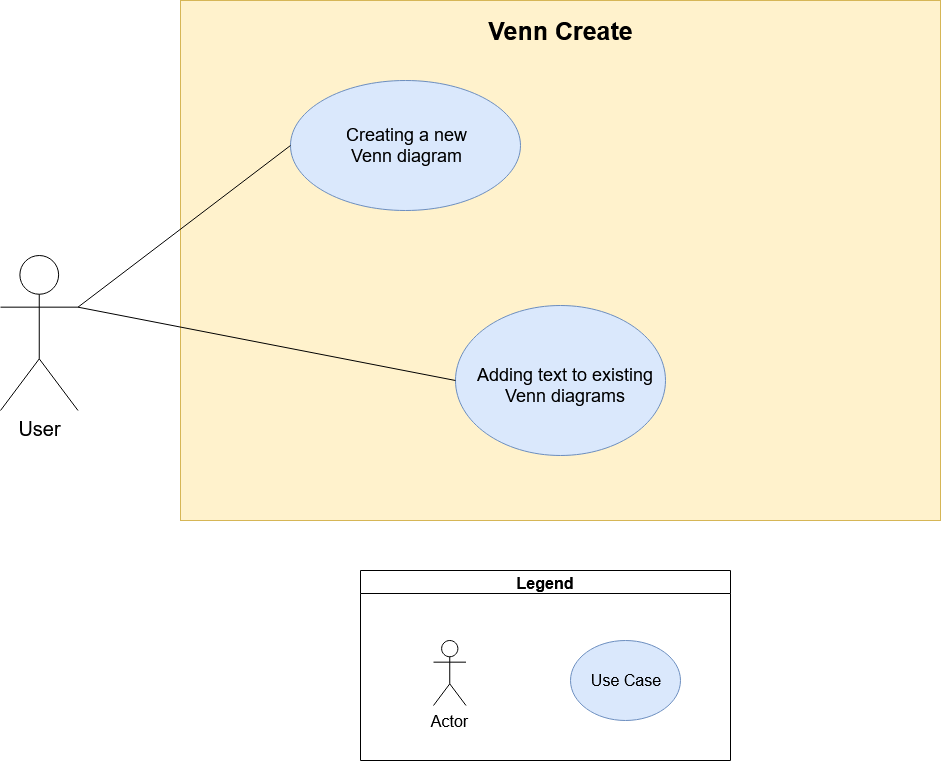
\includegraphics[width=\textwidth]{images/use-case-diagram.png}
	\end{mdframed}
	\caption{Use Case Diagram}
\end{figure}

\newpage

\subsection*{Use Case Textual Description 1}

\begin{table}[h]
	\begin{tabular}{|l|}
		\hline
		\\
		Use case at1: Creating a Venn Diagram													\\
		\\
		This use case describes the operation of a user creating a new Venn diagram 			\\
		to the application. 																\\
		\\
		\underline{Related System Goals}: G1												\\
		\\
		\underline{Primary Actor}: User														\\
		\\
		\underline{Precondition}:															\\ \qquad
		User have already opened the application. 											\\
		\\
		\underline{Postcondition}:															\\ \qquad
		A new Venn diagram has been added to the application.								\\
		\\
		\underline{Main success scenario}:													\\
		\begin{minipage}{6in}
			\vskip 4pt
			\begin{enumerate}
				\item The user may first familiarize themselves with the user interface
						of the program.
				\item When ready the user will click the button Create New.
			\end{enumerate}
			\vskip 4pt
		\end{minipage}
		\\
		\hline
	\end{tabular}
\end{table}

\newpage

\subsection*{Use Case Textual Description 2}

\begin{table}[h]
	\begin{tabular}{|l|}
		\hline
		\\
		Use case at2: Adding text label to existing Venn diagrams.							\\
		\\
		Given that a Venn diagram has been added to the application, this Use Case		\\
		describes how a user add a text label to an existing Venn diagram.					\\
		\\
		\underline{Related System Goals}: G1, G2												\\
		\\
		\underline{Primary Actor}: User														\\
		\\
		\underline{Precondition}:															\\ \qquad
		A Venn diagram exists in the application.								\\
		\\
		\underline{Postcondition}:															\\ \qquad
		A text label is added to the existing Venn diagram.									\\
		\\
		\underline{Main success scenario}:													\\
		\begin{minipage}{6in}
			\vskip 4pt
			\begin{enumerate}
				\item User clicks the show button on the left side of the screen to display the side bar.
				\item User type in the content of the new text label to be added.
				\item User clicks the Add button.
				\item The text label is added to the current Venn diagram.
			\end{enumerate}
			\vskip 4pt
		\end{minipage}
		\\
		\hline
	\end{tabular}
\end{table}

\newpage

\subsection*{Use Case Textual Description 3}

\begin{table}[h]
	\begin{tabular}{|l|}
		\hline
		\\
		Use case at3: Importing existing Venn diagram to the software.							\\
		\\
		Given that at least one saved Venn diagram exists in the local filesystem, this Use Case		\\
		describes how a user can import existing Venn diagram to the software.					\\
		\\
		\underline{Related System Goals}: G1, G2											\\
		\\
		\underline{Primary Actor}: User														\\
		\\
		\underline{Precondition}:															\\ \qquad
		At least one saved Venn diagram exists in the local filesystem							\\ \qquad
		User have already opened the application.											\\
		\\
		\underline{Postcondition}:															\\ \qquad
		A saved Venn diagram is imported to the software.									\\
		\\
		\underline{Main success scenario}:													\\
		\begin{minipage}{6in}
			\vskip 4pt
			\begin{enumerate}
				\item User clicks the Get Existing button on the home page. 
				\item User choose and open a Venn diagram saved file from local filesystem.
				\item The saved Venn diagram is imported to the software.	
			\end{enumerate}
			\vskip 4pt
		\end{minipage}
		\\
		\hline
	\end{tabular}
\end{table}

\newpage

\subsection*{Use Case Textual Description 4}

\begin{table}[h]
	\begin{tabular}{|l|}
		\hline
		\\
		Use case at4: Enters Test Mode and Testing.							\\
		\\
		Given that at least one test file exists in the local filesystem, this Use Case		\\
		describes how a user test the software using Test Mode.					\\
		\\
		\underline{Related System Goals}: G1  											\\
		\\
		\underline{Primary Actor}: User														\\
		\\
		\underline{Precondition}:															\\ \qquad
		At least one test file exists in the local filesystem							\\ \qquad
		User have already opened the application.											\\
		\\
		\underline{Postcondition}:															\\ \qquad
		Test file has been loaded to the software.									\\
		\\
		\underline{Main success scenario}:													\\
		\begin{minipage}{6in}
			\vskip 4pt
			\begin{enumerate}
				\item User clicks the Test Mode on the home page. 
				\item User clicks the IMPORT TXT FILE on the bottom of the software. 
				\item User choose and open a test file from local filesystem.
				\item The Test file has been loaded to the software.	
			\end{enumerate}
			\vskip 4pt
		\end{minipage}
		\\
		\hline
	\end{tabular}
\end{table}

%%%%%%%%%%%%%%%%%%%%%%%%%%%%%%%%%%%%%%%%%%%%%%%%%%%%%%%%%%%%%%%%%%%%%%%%%
\newpage
\section{E-Descriptions: Environmental Constraints}

\reqm{ENV}{The software will run on desktop computers.\\}
{Traceability reference: see Purpose.}

\reqm{ENV}{The software will run on computers with Java 1.8 installed.\\}
{Traceability reference: see Purpose.}

%%%%%%%%%%%%%%%%%%%%%%%%%%%%%%%%%%%%%%%%%%%%%%%%%%%%%%%%%%%%%%%%%%%%%%%%%
\newpage

\section{R-Descriptions: Functional Requirements}

\reqm{REQ}{User shall be able to add new Venn diagrams to the application.\\}
{Traceability reference: see High level goals, Purpose and acceptance test at1.}

\reqm{REQ}{User shall be able to add text labels to the existing Venn diagrams.\\}
{Traceability reference: see High level goals, Purpose and acceptance test at2.}

\reqm{REQ}{User shall be able to export current Venn diagrams to a file.\\}
{Traceability reference: see Purpose.}

\reqm{REQ}{User shall be able to import existing Venn diagrams from a saved file.\\}
{Traceability reference: see Purpose.}

\reqm{REQ}{The software must allow the users to select multiple objects at once in order to customize them, e.g. select all objects in the intersection, and increase their font size.\\}
{Traceability reference: see New requirements added on February 26.}

\reqm{REQ}{The software must implement an Undo/Redo mechanism.\\}
{Traceability reference: see New requirements added on February 26.}

\reqm{REQ}{Each element in the Venn diagram may have a longer description that is by default hidden, but the user must be able to display it.\\}
{Traceability reference: see Stakeholder requirements added on March 3.}

\reqm{REQ}{The software must support a mode where the user is asked to arrange a set of tags on the Venn diagram. Once finished, the user can compare their arrangement to a previously hidden correct answer.\\}
{Traceability reference: see Stakeholder requirements added on March 3.}

%%%%%%%%%%%%%%%%%%%%%%%%%%%%%%%%%%%%%%%%%%%%%%%%%%%%%%%%%%%%%%%%%%%%%%%%%
\newpage
\section{User Interface}

This is the home page of Venn Create, when user first open the software.

\begin{figure}[hbt]
	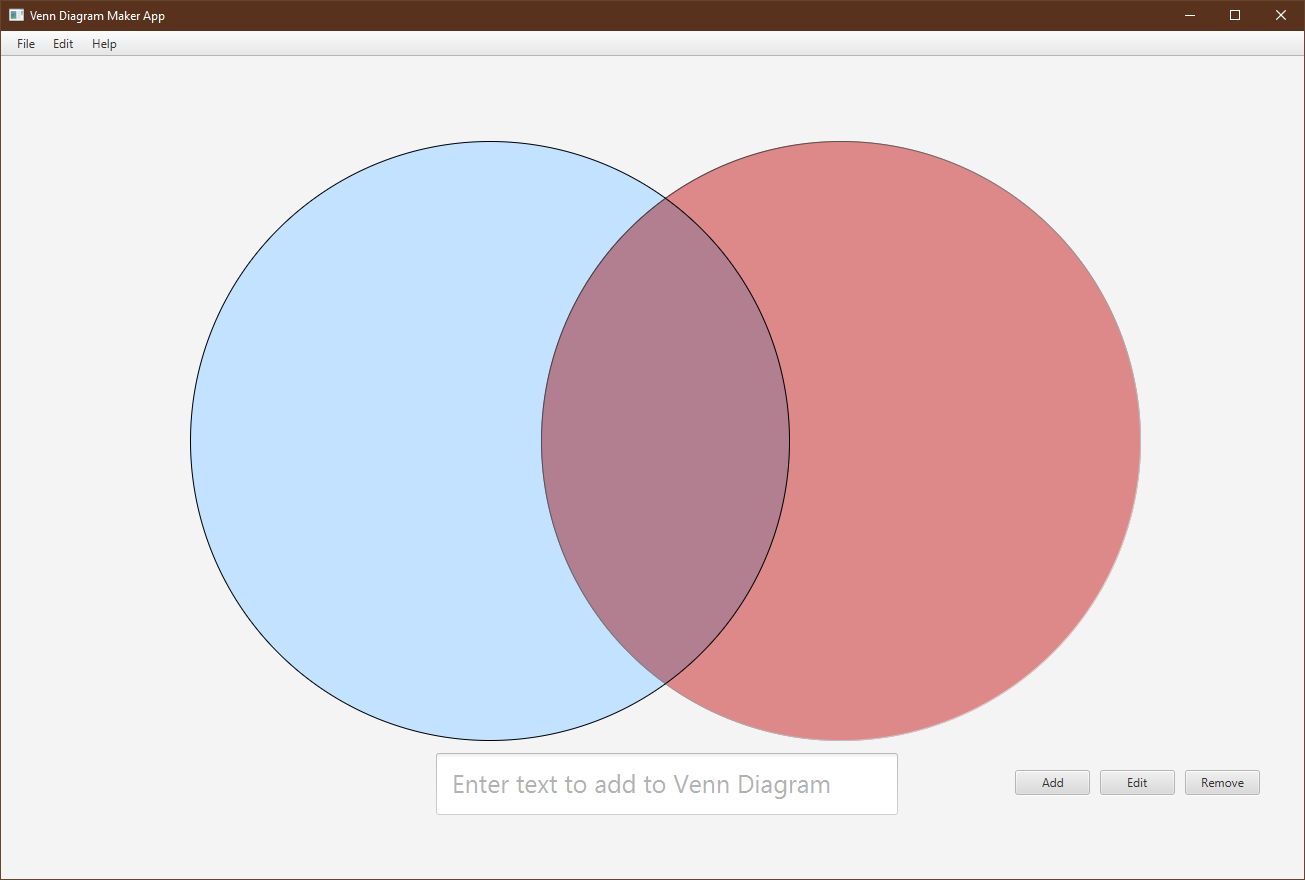
\includegraphics[width=\textwidth]{images/user-interface.png}
	\caption{Home Page of Venn Create}
\end{figure}

\newpage

\subsection{Main UI}

This is the main User Interface of Venn Create, where user can interact with the software by adding new text labels, import, export, adding new circle etc.

This interface will show if the user clicks the Create New button shown above on the home page.

\begin{figure}[!hbt]
	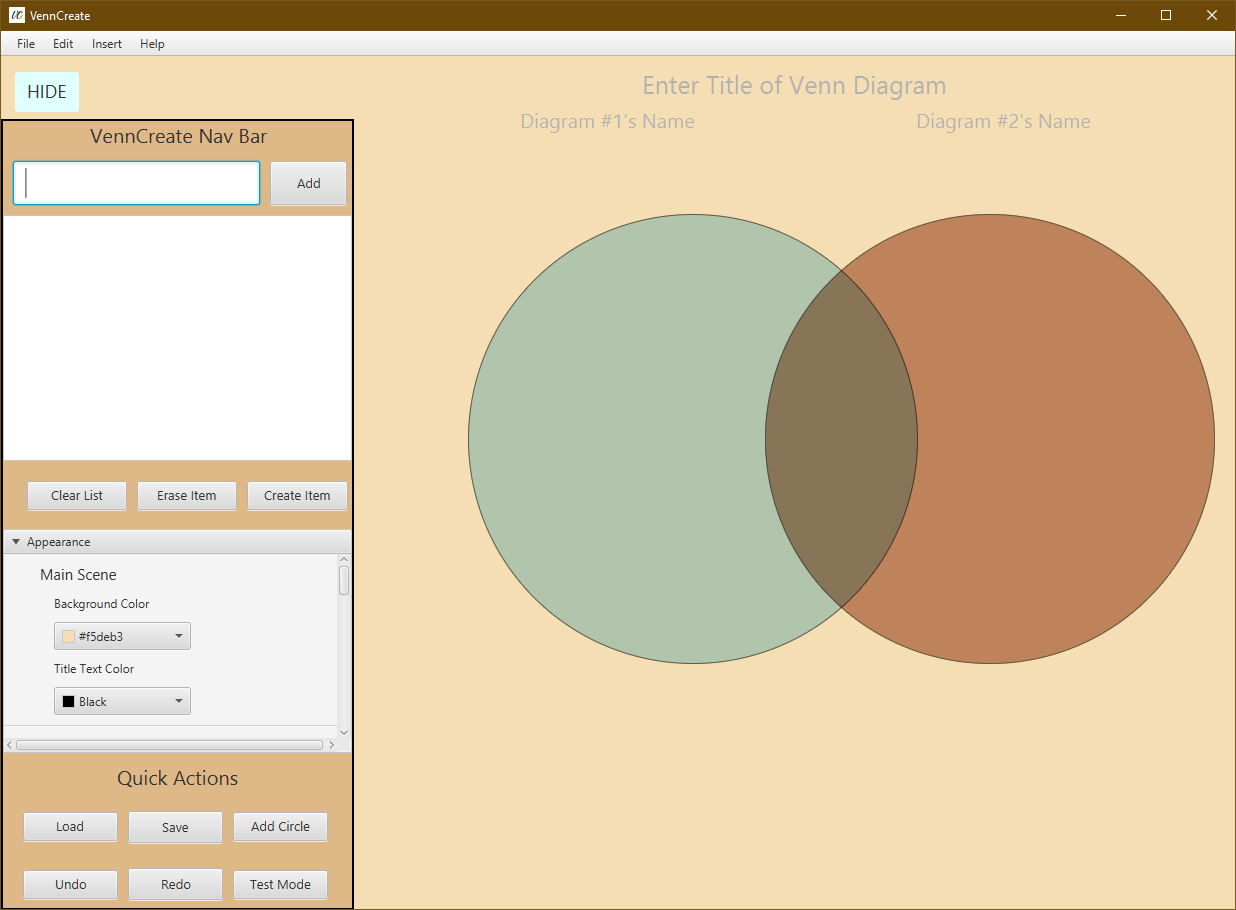
\includegraphics[width=\textwidth]{images/user-interface-normal.png}
	\caption{Main User Interface of Venn Create}
\end{figure}

\newpage

\subsection{Test Mode}

This is the Test Mode of Venn Create, which can be accessed if user clicked Test Mode button on the home page.

In this mode users can import a .txt file with information that they would like to be “tested” on and VennCreate will give them a test.

\begin{figure}[!hbt]
	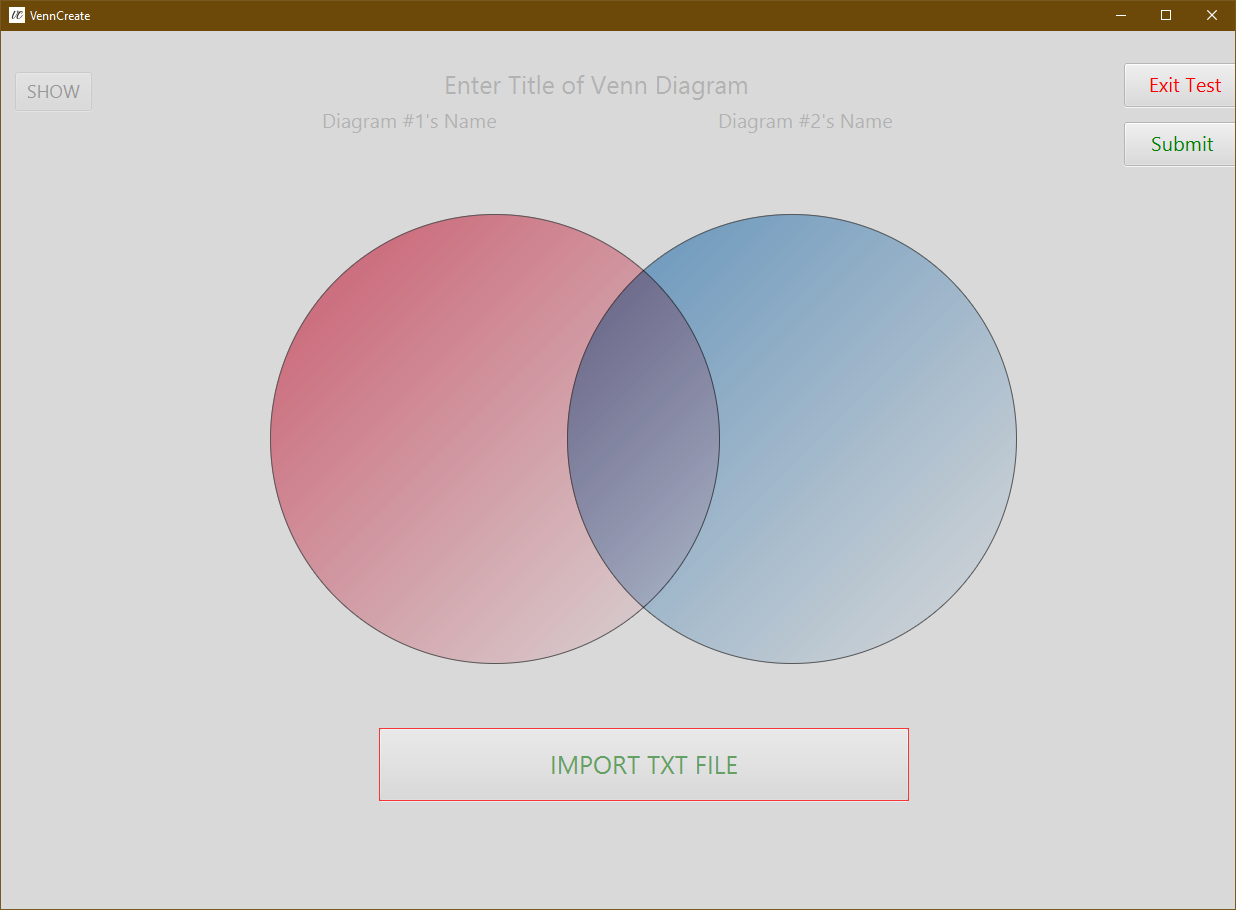
\includegraphics[width=\textwidth]{images/user-interface-test-mode.png}
	\caption{Test Mode User Interface of Venn Create}
\end{figure}

%%%%%%%%%%%%%%%%%%%%%%%%%%%%%%%%%%%%%%%%%%%%%%%%%%%%%%%%%%%%%%%%%%%%%%%%
\newpage
\section{Acceptance Tests}

The table below describes the relationship between our use cases and concrete acceptance tests.

\begin{table}[!ht]
	\centering
	\begin{tabular}{|l|l|l|}
		\hline
		\multicolumn{1}{|c|}{\textbf{Use Cases}} & \multicolumn{1}{c|}{\textbf{Description}}                                    & \multicolumn{1}{c|}{\textbf{Acceptance Tests}} \\ \hline
		UC1                                      & Creating a Venn diagram                  & at1                                            \\ \hline
		UC2                                      & Adding a text label to existing Venn diagrams.                        			     & at2                                            \\ \hline
		UC3                                      & Importing existing Venn diagram to the software.                        			     & at3                                            \\ \hline
		UC4                                      & Enters Test Mode and Testing.                        			     & at4                                            \\ \hline
	\end{tabular}
	\caption{Acceptance Tests for each Use Case}
	\label{acceptance-tests}
\end{table}

The following pages contain detailed descriptions of all the acceptance tests.

\newpage

\begin{table}[!h]
	\begin{tabular}{|l|}
		\hline
		\\
		\textbf{\emph{Acceptance Test at1}} 	
		\\\\
		\underline{Purpose}: Testing the creating a new Venn diagram functionality						\\
		\\
		\underline{Category}: Basic															\\
		\\
		\underline{Precondition}:															\\ \qquad
		User has successfully opened the application.										\\
		\\
		\underline{Reproduction Steps:}
		\\ \qquad 1. In the main menu, click 'Create New'.
		\\ \qquad \textit{Result: the main user interface will be displayed with a new Venn diagram}
		\\ \qquad \qquad \qquad \textit{created.}
		\\\\
		\hline
	\end{tabular}
\end{table}

\newpage

\begin{table}[!h]
	\begin{tabular}{|l|}
		\hline
		\\
		\textbf{\emph{Acceptance Test at2}} 	
		\\\\
		\underline{Purpose}: Testing the add text label to existing Venn diagram functionality \\
		\\
		\underline{Category}: Basic		\\
		\\
		\underline{Precondition}:															\\ \qquad
		User has successfully opened the application.
		\\ \qquad
		A Venn diagram exists in the application.
		\\\\
		\underline{Reproduction Steps}:				
		\\\\ \qquad 1. Click the 'show' button on the top left of the screen.
		\\ \qquad \textit{Result: the VennCreate Nav Bar will be displayed .} 
		\\\\ \qquad 2. Type 'Foo' to the text field.
		\\ \qquad \textit{Result: Text field should now display 'Foo'.} 
		\\\\ \qquad 3. Click the 'Add' button on the right side of the text field.
		\\ \qquad \textit{Result: A text label contains 'Foo' is added to Venn Diagram.} 
		\\\\
		\hline
	\end{tabular}
\end{table}

\newpage

\begin{table}[!h]
	\begin{tabular}{|l|}
		\hline
		\\
		\textbf{\emph{Acceptance Test at3}} 	
		\\\\
		\underline{Purpose}: Testing import existing saved Venn diagram functionality \\
		\\
		\underline{Category}: Advanced		\\
		\\
		\underline{Precondition}:															\\ \qquad
		User has successfully opened the application.
		\\ \qquad
		A Venn diagram saved file exists in the filesystem.
		\\\\
		\underline{Reproduction Steps}:				
		\\\\ \qquad 1. In the main menu, click the 'Get Existing' button.
		\\ \qquad \textit{Result: a file chooser will pop-up.} 
		\\\\ \qquad 2. Choose and open the saved file using the file chooser.
		\\ \qquad \textit{Result: The file chooser disappears and the saved Venn diagram is loaded.} 
		\\\\
		\hline
	\end{tabular}
\end{table}

\newpage

\begin{table}[!h]
	\begin{tabular}{|l|}
		\hline
		\\
		\textbf{\emph{Acceptance Test at4}} 	
		\\\\
		\underline{Purpose}: Testing Test Mode and import test file functionality \\
		\\
		\underline{Category}: Advanced		\\
		\\
		\underline{Precondition}:															\\ \qquad
		User has successfully opened the application.
		\\ \qquad
		A test file exists in the filesystem.
		\\\\
		\underline{Reproduction Steps}:				
		\\\\ \qquad 1. In the main menu, click the 'Test Mode' button.
		\\ \qquad \textit{Result: the software will enter Test Mode.} 
		\\\\ \qquad 2. Click the 'IMPORT TXT FILE' button on the bottom of the screen.
		\\ \qquad \textit{Result: a file chooser will pop-up.} 
		\\\\ \qquad 3. Choose and open the test file using the file chooser.
		\\ \qquad \textit{Result: The file chooser disappears and the test case is loaded.} 
		\\\\
		\hline
	\end{tabular}
\end{table}

\newpage

\begin{table}[!h]
	\begin{tabular}{|l|}
		\hline
		\\
		\textbf{\emph{Acceptance Test at5}} 	
		\\\\
		\underline{Purpose}: Testing export current Venn diagram functionality \\
		\\
		\underline{Category}: Advanced		\\
		\\
		\underline{Precondition}:															\\ \qquad
		User has successfully opened the application.
		\\ \qquad
		A Venn diagram exists in the application.
		\\\\
		\underline{Reproduction Steps}:				
		\\\\ \qquad 1. Click the 'show' button on the top left of the screen.
		\\ \qquad \textit{Result: the VennCreate Nav Bar will be displayed .} 
		\\\\ \qquad 2. Click the 'SAVE' button under section Quick Actions.
		\\ \qquad \textit{Result: a dialogue should pop-up asking the title of the project.} 
		\\\\ \qquad 3. Enter 'Foo' input the text field and clicks Ok button.
		\\ \qquad \textit{Result: A file chooser should pop-up asking the location to save the file.} 
		\\\\ \qquad 4. Choose a desired place and click the confirm button.
		\\ \qquad \textit{Result: The file chooser disappears and the diagram has been saved.} 
		\\\\
		\hline
	\end{tabular}
\end{table}

\newpage

\begin{table}[!h]
	\begin{tabular}{|l|}
		\hline
		\\
		\textbf{\emph{Acceptance Test at6}} 	
		\\\\
		\underline{Purpose}: Testing editing and customizing text labels in the Venn diagram \\
		\\
		\underline{Category}: Advanced		\\
		\\
		\underline{Precondition}:															\\ \qquad
		User has successfully opened the application.
		\\ \qquad
		A Venn diagram exists in the application.
		\\ \qquad
		At least one text label exists in the Venn diagram.
		\\\\
		\underline{Reproduction Steps}:				
		\\\\ \qquad 1. Click the 'show' button on the top left of the screen.
		\\ \qquad \textit{Result: the VennCreate Nav Bar will be displayed.} 
		\\\\ \qquad 2. In the 'Appearance' section, scroll down to the option 'Font Size'.
		\\ \qquad \textit{Result: 'Font Size' option should be visible on screen.} 
		\\\\ \qquad 3. Drag the slide bar under 'Font Size' to '11'.
		\\ \qquad \textit{Result: The font size of all the text labels in the Venn diagram changed to 11.} 
		\\\\ \qquad 4. Right click one of the text labels in the Venn diagram and select
		\\ \qquad \qquad 'Add longer description'.
		\\ \qquad \textit{Result: A dialogue should pop-up asking the description to be put in.} 
		\\\\ \qquad 5. Enter 'Foo' input the text box and click 'Ok'.
		\\ \qquad \textit{Result: The description should be added to the text label.} 
		\\\\
		\hline
	\end{tabular}
\end{table}

\newpage

\begin{table}[!h]
	\begin{tabular}{|l|}
		\hline
		\\
		\textbf{\emph{Acceptance Test at7}} 	
		\\\\
		\underline{Purpose}: Testing Undo/Redo mechanism \\
		\\
		\underline{Category}: Advanced		\\
		\\
		\underline{Precondition}:															\\ \qquad
		User has successfully opened the application.
		\\ \qquad
		A Venn diagram exists in the application.
		\\ \qquad
		At least one text label exists in the Venn diagram.
		\\\\
		\underline{Reproduction Steps}:				
		\\\\ \qquad 1. Right click one of the text labels in the Venn diagram and select 'Delete'.
		\\ \qquad \textit{Result: selected text label is deleted.} 
		\\\\ \qquad 2. In the menu bar, click 'Edit', and then 'Undo'.
		\\ \qquad \textit{Result: the deleted text label is recovered.} 
		\\\\
		\hline
	\end{tabular}
\end{table}
%%%%%%%%%%%%%%%%%%%%%%%%%%%%%%%%%%%%%%%%%%%%%%%%%%%%%%%%%%%%%%%%%%%%%%%%
\newpage
\section{Traceability Matrix}

The following table outlines which R-descriptions are tested by which acceptance tests.

\begin{table}[!ht]
	\centering
	\begin{tabular}{|l|l|l|l|l|l|l|l|}
		\hline
		\textbackslash{}textbf\{REQ\} & at1 & at2 & at3 & at4 & at5 & at6 & at7 \\ \hline
		REQ3                          & X   &     &     &     &     &     &     \\ \hline
		REQ4                          &     & X   &     &     &     &     &     \\ \hline
		REQ5                          &     &     &     &     & X   &     &     \\ \hline
		REQ6                          &     &     & X   &     &     &     &     \\ \hline
		REQ7                          &     &     &     &     &     & X   &     \\ \hline
		REQ8                          &     &     &     &     &     &     & X   \\ \hline
		REQ9                          &     &     &     &     &     & X   &     \\ \hline
		REQ10                         &     &     &     & X   &     &     &     \\ \hline
	\end{tabular}
	\caption{Traceability matrix for R-descriptions}
	\label{tbl:at}
\end{table}
%%%%%%%%%%%%%%%%%%%%%%%%%%%%%%%%%%%%%%%%%%%%%%%%%%%%%%%%%%%%%%%%%
\end{document} 	

